% Section 1 of the theory paper (adr/0007): the introduction, written for the theory alone, and
% section 1.1, which owns the trust base (article-kit WRITING.md section 4). Statement numbers are
% \ref'd, never typed; the computation paper is unreleased and is named only as further work.
\section{Introduction}
\label{sec:intro}

An image pyramid stores an image at a sequence of resolutions. Each level is a smoothed copy of the
one before, subsampled by a fixed ratio $q$, usually $2$ \cite{burt1981fast,burt1983laplacian}. The
design literature constrains the generating kernel of one step. Burt and Adelson require it to be
separable, normalized, symmetric and of equal contribution \cite[p.~533]{burt1983laplacian}. Meer,
Baugher and Rosenfeld judge it by its distance from the ideal low-pass filter for decimation by $2$,
measured by the share of the spectrum folded back and by the error in the passband
\cite[pp.~513--515]{meer1987frequency}. Burt
observed that the equivalent kernels of the levels approach one shape \cite{burt1981fast}. What the
literature does not state is a property of the whole family of kernels: every level looks like every
other on its own grid. As an axiom, this is covariance under the dilations by $q^n$, $n \in \ZZ$,
which leaves every other dilation optional.

Scale-space theory supplies the rest. Its classical axioms require a semigroup of linear smoothings,
$\Phi_{t+s} = \Phi_t\Phi_s$ \cite[\S 3, Axiom~6, p.~270]{duits2004axioms},
\cite[\S 2.4.4, p.~41]{lindeberg1994scale}, as in Lindeberg's scale space for discrete signals
\cite{lindeberg1990scalespace}. Iijima's axioms, the earliest, require less: two smoothings compose to
a third, of some scale \cite[\S 3, p.~241]{weickert1999linear}.
Lindeberg notes that this theory does not cover pyramids, with their shrinking grids and fixed
sampling of scale. He asks how far a subsampling can enter a scale-space representation and keep the
properties that come from a continuous scale parameter \cite[\S 3.4.1, p.~82; \S 4.5.4,
p.~122]{lindeberg1994scale}.
The author's earlier papers replace the semigroup by a \emph{hemigroup}: a family of operators
$\Phi_{s,t}$ from scale $s$ to scale $t$ in which two consecutive steps compose to one,
$\Phi_{t,u}\Phi_{s,t} = \Phi_{s,u}$. This cascade ties the scale to no additive parameter. With
continuity in scale, symmetry, positivity and covariance under every dilation, the hemigroup axioms
classify the families of kernels on the line \prog{V-line v0.1}{Thm.~7.3, p.~37}, and in $\RR^d$ the
isotropic ones \prog{iso v0.1}{Thm.~3.6, p.~13}. Covariance under every dilation is more than a
pyramid needs, since a pyramid is looked at only at the scales $q^n$. This paper keeps the cascade,
continuity and positivity. It keeps nondegeneracy too, except in Section~\ref{ch:price}, which
requires it of the octave step only. It requires symmetry or rotation invariance where a result needs it,
and covariance at the one ratio $q$ only.

Read in this way, a pyramid samples a scale space. Its levels are the image at the scales $q^n$,
the \emph{knots}, of one family: the input is read as the image at the scale $1$, and level $n$
applies the steps of the family from $1$ to $q^n$. What it computes is the step from each knot to the next, the
\emph{octave step} across a factor $q$ in scale, and the sequence of these steps is the
\emph{ladder} of the family (Figure~\ref{fig:pyramid-schematic}). Burt's observation points to such a
family behind the classical pyramids. For this reading to say something about a given pyramid, two
things must be known. The first is which families there are. The classifications above do not
answer it, because they require covariance under every dilation, and a pyramid tests covariance at
the powers of $q$ only. The second is how much of a family its ladder fixes. A pyramid computes the
ladder and nothing between the knots, so whatever the ladder leaves free is invisible in its output.
Section~\ref{ch:pyramid} settles both in $\RR^d$.

Covariance under one ratio admits many families. Scale-space theory singles out a family by a
principle about what smoothing may do to an image. On the line the principle is the classical one
that smoothing creates no new local extrema. Their number does not grow with scale, and this
selects among the families of the line \prog{V-selection v0.1}{\S4}. Images live in the plane, and
there the principle fails. One octave step of the pyramid of Section~\ref{ch:matern} can raise the number
of local maxima (Figure~\ref{fig:theory-creation}), and so can an octave step of the Gaussian
ladder, at any scale. A pyramid for images
therefore needs a principle that holds in the plane and can be stated on its octave steps.
Section~\ref{ch:matern} gives one, and finds the family it selects.

Finally, a pyramid is computed on a grid. At every level it applies one array of weights, the
\emph{mask}, on the lattice of that level, and from one level to the next the lattice and the mask
are both spread out by the factor $q$. The lattices are nested, $q\Gamma \subseteq \Gamma$, only
when $q$ is an integer, so every statement about decimated records takes $q$ an integer. The
definitions make sense for every $q > 1$. Two properties are wanted of the result. The first is that
the steps it applies from level to level be the octave steps of one family, continuous in scale and
covariant under $q$, so that what is known of families applies to what is computed. Such a pyramid
is called \emph{exact}. The second is that the
pyramid treat every orientation of the image alike. It is called \emph{isotropic} when some kernel of
its family at a positive scale is rotation invariant. The classical masks were designed for neither
property. Section~\ref{ch:price} asks which masks give an exact pyramid, and whether an exact pyramid
can also be isotropic.

\begin{figure}[t]
\centering
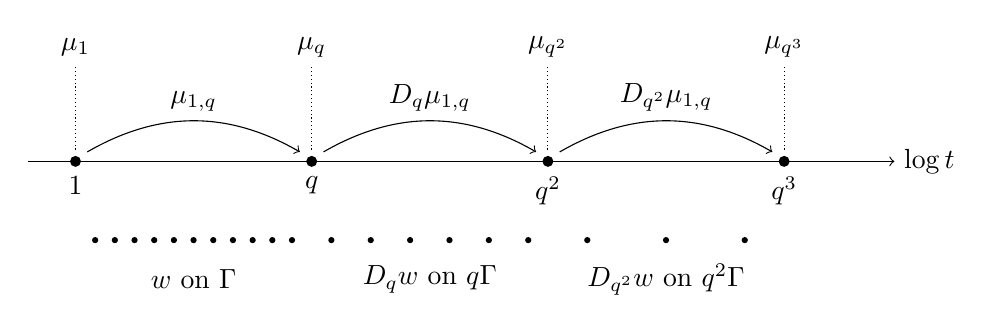
\begin{tikzpicture}[x=1cm,y=1cm,
  knot/.style={circle,fill,inner sep=1.4pt},
  gp/.style={circle,fill,inner sep=0.8pt}]
\draw[->] (-0.6,0) -- (10.4,0) node[right] {$\log t$};
\foreach \x/\lab in {0/1, 3/q, 6/q^2, 9/q^3} {
  \node[knot] at (\x,0) {};
  \node[below=2pt] at (\x,0) {$\lab$};
  \node at (\x,1.45) {$\mu_{\lab}$};
  \draw[densely dotted] (\x,0.15) -- (\x,1.2);
}
\foreach \x/\lab in {0/{\mu_{1,q}}, 3/{D_q\mu_{1,q}}, 6/{D_{q^2}\mu_{1,q}}} {
  \draw[->,bend left=30] (\x+0.15,0.12) to node[above] {$\lab$} (\x+2.85,0.12);
}
\foreach \k in {0,...,10} { \node[gp] at (0.25+0.25*\k,-1.0) {}; }
\foreach \k in {0,...,5} { \node[gp] at (3.25+0.5*\k,-1.0) {}; }
\foreach \k in {0,...,2} { \node[gp] at (6.5+1.0*\k,-1.0) {}; }
\node at (1.5,-1.5) {$w$ on $\Gamma$};
\node at (4.5,-1.5) {$D_qw$ on $q\Gamma$};
\node at (7.5,-1.5) {$D_{q^2}w$ on $q^2\Gamma$};
\end{tikzpicture}
\caption{A pyramid on the scale axis, drawn on a logarithmic scale. Levels are stored at the knots
$q^n$, and the knot kernels $\mu_{q^n}$ stand above them. The octave steps between consecutive
knots form the ladder, each step the dilate of $\mu_{1,q}$ by covariance
(Definition~\ref{def:knots-and-ladder}). Below, a grid pyramid applies one mask $w$ on a lattice
$\Gamma$, dilated to $D_{q^n}w$ on $q^n\Gamma$ at every level
(Definition~\ref{def:exact-grid-pyramid}). It is exact when a family continuous in scale and
covariant under $q$ has these steps as its ladder. Four objects are kept apart: the kernel
$\mu_t = \mu_{0,t}$ from the scale $0$ to $t$, the step $\mu_{s,t}$ from $s$ to $t$, a mask on a
lattice, and the samples of a continuum density. The input on the finest grid is read as the image
at the scale $1$. Level $n$ then applies the steps from $1$ to $q^n$, whose convolution is the
equivalent weight $W_n$ of Proposition~\ref{prop:equivalent-weights}. The knot kernel $\mu_{q^n}$
would also apply the smoothing below the scale $1$.}
\label{fig:pyramid-schematic}
\end{figure}

\paragraph{Contributions.} The answers, each proved in the section named, are the following.
\begin{enumerate}
\item \emph{Which families a pyramid can sample} (Section~\ref{ch:pyramid}). The dilations under
which a symmetric family is covariant form a closed group, so there are three cases: the identity
alone, the powers of one ratio $q$, or every dilation (Lemma~\ref{lem:family-dilations}). For a
fixed ratio $q$ the families therefore form three nested \emph{strata}: every symmetric family
(stratum~1), those covariant under the powers of $q$ (stratum~2), and those covariant under every
dilation (stratum~3). The strata depend on $q$, while the three cases of the group do not. The
pyramids are stratum~2: a \emph{pyramid} here is a family of stratum~2 read at its knots. The
computation that smooths and subsamples is called the computed pyramid, and the ladder of a mask on
a lattice a grid pyramid (Definition~\ref{def:exact-grid-pyramid}). For isotropic families each stratum is described by the
Gaussian part of the kernels and by their \Levy{} measures, which record the jumps, and each stratum
is strictly larger than the next (Theorems~\ref{thm:lattice-strata}
and~\ref{thm:lattice-strata-strict}). An isotropic family is fixed by its marginal on one axis
(Lemma~\ref{lem:reduction-keeps-stratum}). The line does not say which of its families extend to
$\RR^d$. The line's examples of the lower strata do not: in $d \ge 2$ no line exponent with
an atom in its \Levy{} measure is the marginal of a rotation-invariant infinitely divisible law
(Proposition~\ref{prop:what-does-not-lift}). The isotropic classes of one ratio shrink strictly as
the dimension grows (Proposition~\ref{prop:what-does-not-lift-chain}), as the fully covariant ones
do.

In stratum~2 the ladder fixes the kernels at the knots. The kernel at a knot is the convolution of all
the rungs below it, a limit, which is Burt's equivalent weighting function run downward in scale. The kernels between the knots are not fixed by the ladder. A
symmetric law other than a point mass is the octave step of such a family exactly when it is
infinitely divisible and has a logarithmic moment, $\int\log_+|x|\,\varrho(dx) < \infty$
(Proposition~\ref{prop:ladder-knot-kernel}). A law is \emph{infinitely divisible} when, for every
$n$, it is the $n$-fold convolution power of some law (Section~\ref{subsec:cited-sato}). For laws
this criterion is a theorem of Maejima and Ueda \cite[Thm.~3.3, p.~353]{maejima2009stochastic}. No law of
bounded support other than a point mass is a step $\mu_{s,t}$ of any family. The cascade and
continuity in scale exclude it, with no symmetry, covariance or nondegeneracy assumed
(Proposition~\ref{prop:no-bounded-step}). The proof joins two facts. The steps of a family are
infinitely divisible (Lemma~\ref{lem:steps-infinitely-divisible}; for processes
\cite[Thm.~9.1, p.~47]{sato1999levy}), and an infinitely divisible law other than a point mass has
unbounded support (Theorem~\ref{thm:cited-A46}). So the finite masks of the classical pyramids are the
octave steps of no family. A nonnegative one is excluded by that proposition. One with a negative
weight is excluded from the start, since every step of a family is a probability law.

\item \emph{The line and its grids} (Section~\ref{sec:line-theory}). On a grid $h\ZZ$ the criterion
becomes a criterion for masks: a symmetric probability mask other than $\delta_0$ has an exact
pyramid exactly when it is infinitely divisible
with a logarithmic moment, and the kernel at the knots is then unique. Continuity in scale forces
the infinite divisibility, through the steps of the family. Such a pyramid lies in
stratum~2 and never in stratum~3, since no family covariant under every dilation has a symmetric
lattice law other than $\delta_0$ as a step. The sampled Laplace mask, the two-sided exponential
density sampled on the grid, has an exact pyramid for every $q > 1$. No mask of bounded support has
one, the binomial and B-spline masks among them
(Proposition~\ref{prop:grid-pyramids-infinitely-divisible}). The sampled Laplace mask is applied by
one forward and one backward first-order recursion. For a fixed spacing, the sampled Laplace
kernels form an \emph{exact cascade} on the grid: the step between any two of them is again a
positive grid kernel of unit mass. This is a use of the word outside the three senses of
Definition~\ref{def:exact-senses}, which are these:
(i) a computation whose arrays are the kernels they stand for;
(ii) a family of grid kernels in which every $q$-th value of a member, renormalized, is a member;
(iii) a pyramid whose ladder is that of a continuous covariant family.
The word \emph{exact} in \emph{exact grid pyramid} is sense (iii). For an integer $q \ge 2$, the \Matern{} pyramid of
Section~\ref{ch:matern} computed by these recursions with decimation equals the samples of its
continuum steps at the first level, and differs from them at every later level, for every spacing
(Proposition~\ref{prop:sampled-laplace-exact}).

\item \emph{The \Matern{} pyramid and its selection} (Section~\ref{ch:matern}). The principle that
replaces the count of extrema is the maximum principle of an implicit Euler step of the heat
equation. At a local maximum of the output, the output does not exceed the input. At a local
minimum it is not below it (Definition~\ref{def:implicit-euler-principle}). Label the scales so that dilating
the kernel at $t$ by $q$ gives the kernel at $qt$. Required of every octave step, from every scale $t$ to $qt$, and for every smooth rapidly decreasing input, the principle singles out
one isotropic family covariant under $q$, up to a relabelling in the group $\mathcal{G}_q$ of
Lemma~\ref{lem:family-dilations}(3), which keeps that labelling. This is the \emph{\Matern{} pyramid}
(Theorem~\ref{thm:selection-stratum-two}(2)). In the labelling of Theorem~\ref{thm:matern-pyramid}, its octave step from $t$ to $qt$ is one implicit Euler
step of the heat equation, the Bessel potential $(I - c^2t^2\Delta)^{-1}$ with a constant $c > 0$,
so the step size grows by $q^2$ per octave (Theorem~\ref{thm:matern-pyramid}). The selected family
is covariant under every dilation (Theorem~\ref{thm:matern-pyramid}(1)). So it lies in stratum~3,
among the families that the isotropic paper classifies, although only covariance under $q$ was
required. The difference of the
levels $t$ and $qt$ is $-c^2t^2$ times the Laplacian of the coarser one. So for this family the
Laplacian pyramid of Burt and Adelson, read on the continuum before decimation, is a Laplacian
(Proposition~\ref{prop:laplacian-pyramid}). The selection rests on the stage lemma: a
rotation-invariant law other than $\delta_0$ that has the principle is a Bessel potential
(Proposition~\ref{prop:stage-lemma}). Among symmetric rotation-invariant laws the principle
therefore holds exactly for the Bessel potentials, and every Gaussian step fails it (Theorem~\ref{thm:selection-stratum-two}(4)). The
principle is a property of one step, and the theorem requires it of the octave steps only. A step
of the \Matern{} pyramid from $s$ to $t$ has it only when $t = qs$
(Theorem~\ref{thm:selection-stratum-two}(3)), and no symmetric family has it at every step
(Proposition~\ref{prop:principle-other-readings}(2)). The count of extrema does not select among the families with
absolutely continuous steps in the plane, since one step of every absolutely continuous law can
create a local maximum
(Proposition~\ref{prop:creation-plane}).

\item \emph{Exact pyramids on a lattice in $d \ge 2$ are not isotropic} (Section~\ref{ch:price}). In every dimension, a
symmetric probability mask on a lattice, other than a point mass, has an exact pyramid exactly when it is
infinitely divisible with a logarithmic moment (Proposition~\ref{prop:exact-masks}). The
criterion does not involve $q$, so exactness is a property of the mask alone. Such a mask has
unbounded support, so a pyramid that truncates its mask is not exact. The resolvent masks of the
discrete Helmholtz operators meet the criterion (Proposition~\ref{prop:resolvent-masks-exact}). In
$d \ge 2$ no exact pyramid whose mask is carried by a lattice is isotropic
(Proposition~\ref{prop:grid-pyramid-not-isotropic}). The same holds when the dilation is an
invertible matrix, which may also turn the lattice, as in the quincunx and hexagonal pyramids
(Proposition~\ref{prop:expanding-grid-pyramid-not-isotropic}). The reason
is where the jumps lie. An infinitely divisible lattice law has no Gaussian part, and its \Levy{}
measure lies on the lattice (Lemma~\ref{lem:lattice-infinitely-divisible}). Through the knot
product the same holds for the family: every kernel at a positive scale has no Gaussian part and a
nonzero \Levy{} measure carried by a countable set
(Proposition~\ref{prop:grid-pyramid-not-isotropic}(1)). In $d \ge 2$ a rotation-invariant law with
a nonzero \Levy{} measure cannot be carried that way. So in $d \ge 2$ no kernel at a positive scale
of any family carrying an exact pyramid on a lattice is rotation invariant
(Proposition~\ref{prop:grid-pyramid-not-isotropic}(2)), and no such pyramid is isotropic. The
obstruction needs continuity in scale as well as the lattice. For a mask with an exponential
moment, as every finite mask has, the knot relation
$D_q\mu_1 = \mu_1 * w$ alone excludes isotropy: its only rotation-invariant solution is $\delta_0$
(Proposition~\ref{prop:no-isotropic-refinable-finite-mask}). For some masks of infinite support it
does not, and no family continuous in scale carries those masks
(Proposition~\ref{prop:band-limited-refinable-mask}).
Isotropy
is defined through a carrying family, so a grid pyramid without one is not isotropic in this sense
either. The continuum \Matern{} pyramid,
with no lattice, is isotropic.

Exact pyramids on a lattice exist in every dimension. One is the frame \Matern{} pyramid on the
grid, whose mask is the product of sampled Laplace masks along the coordinate axes
(Proposition~\ref{prop:grid-pyramid-not-isotropic}). In $d \ge 2$ its mask fails the implicit-Euler
principle on every finite symmetric neighbourhood, while each pass along one axis has it on every
such neighbourhood that contains the two neighbours on that axis
(Proposition~\ref{prop:grid-frame-step-not-selected}). Local maxima are created on the grid as well.
Read them on a finite symmetric neighbourhood that contains the axis neighbours. Then, in $d \ge 2$
and for an integer $q \ge 2$, three masks each create a local maximum across one level of the
decimated pyramid, at every level, for an input that depends on the level: the frame mask, the resolvent mask of the $(2d+1)$-point
Laplacian, and the tensor power of the binomial mask (Propositions~\ref{prop:creation-grid-masks}
and~\ref{prop:binomial-records}). The section ends with the resolvent kernels of the
$(2d+1)$-point Laplacian on $h\ZZ^d$ and of the nine-point Laplacian on $h\ZZ^2$, whose convolution
powers form exact cascades on the grid (Propositions~\ref{prop:discrete-helmholtz}
and~\ref{prop:nine-point-family}).
\end{enumerate}

\paragraph{Relation to the literature.} Each octave of the \Matern{} pyramid is one implicit heat
step, and the step sizes grow geometrically. Such sequences of implicit steps occur in nonstationary
iterated Tikhonov regularization \cite[pp.~38--39]{hanke1998nonstationary}, read there as diffusion time in
\cite[p.~98]{radmoser2000scale}, and in multiscale edge-preserving decompositions
\cite[\S 3.1, (13)--(14)]{farbman2008edge}. Scherzer and Weickert read one regularization step as
one implicit diffusion step and prove its extremum principle
\cite[p.~43; Lemma~6, p.~53]{scherzer2000relations}.
Nielsen, Florack and Deriche read the first-order regularization filter as the heat equation with a
remapped scale, and compute products of such filters recursively
\cite[pp.~296--298]{nielsen1997regularization}.
Decimation between the implicit steps, a covariant family through them, and its uniqueness up to
the gauge under the implicit-Euler principle were not found in that literature. Decimation between explicit steps is Burt's \cite[\S 4, p.~29]{burt1981fast}. The
covariance condition under one ratio is, for laws, semi-selfdecomposability
\cite[Def.~3.1, p.~19]{maejima1998semi}, \cite[Def.~15.1, p.~90]{sato1999levy}, and the strata are
its reading for scale spaces. In probability theory two-parameter families of laws with the
cascade are called convolution hemigroups. Becker-Kern treats those covariant under a linear map,
at every ratio and at the powers of one ratio \cite[p.~574]{becker-kern2003stable}. For laws, the criterion for an octave step, an infinitely divisible
law with a logarithmic moment, is a theorem of Maejima and Ueda on semi-selfdecomposable laws of one
span \cite[Thm.~3.3, p.~353]{maejima2009stochastic}. This paper adds its reading as the ladder of a
family, the kernels between the knots, and their use in the selection. Multiresolution analysis \cite[(2)--(8), p.~676]{mallat1989theory} is the axiomatic dyadic
neighbour, by projection rather than smoothing. Lindeberg's scale space for discrete signals
\cite{lindeberg1990scalespace} lies in stratum~1 and not in stratum~2: it is covariant under no
dilation (Section~\ref{sec:line-theory}). Lindeberg's time-causal limit kernel is an infinite
convolution of first-order integrators whose time constants fall in a fixed ratio, his distribution
parameter. It is covariant under the integer powers of that ratio
\cite[\S 5, p.~62; (47), p.~63]{lindeberg2016time}. It is
the nearest precedent in scale-space theory for covariance under one ratio. On the line the kernel
$\mu_t$ of the \Matern{} pyramid is the limit kernel of ratio $q$ and time constants $ctq^{-i}$,
$i \ge 1$, convolved with its reflection. In every dimension $\mu_t$ is a mixture of Gaussians whose
variance has the law of the limit kernel of ratio $q^2$ (Section~\ref{ch:matern}). The \Matern{} pyramid takes its name from the \Matern{}
covariances, whose transforms are powers of the transform of its octave step [\sscite{whittle1954stationary}, p.~448; \sscite{lindgren2011explicit}, (2), p.~426].
Lowe's pyramid of scale-invariant features smooths by Gaussian steps of ratio $2^{1/s}$ within each
octave and subsamples by $2$ between octaves \cite[pp.~6--7]{lowe2004distinctive}. Read as in this
paper, it computes the steps of the Gaussian family, with sampled kernels. Lindeberg's discrete
approximations of Gaussian smoothing leave subsampling aside \cite[p.~762]{lindeberg2024discrete}.
Other pyramids change the ratio or the smoothing. Crowley resamples by $\sqrt2$, onto a lattice
turned by $45^\circ$ \cite[\S 3.3.2, p.~32]{crowley1981representation}. The hybrid pyramids of
Lindeberg and Bretzner take several smoothing steps between two subsamplings by~$2$
\cite[\S 3.1]{lindeberg2003real}. The polynomial spline pyramids of Unser, Aldroubi and Eden reduce
and expand with binomial filters, and for cubic splines they are close to Burt's
\cite[\S IV.B, p.~370]{unser1993polynomial}.
That Gaussian smoothing can create a local extremum in the plane is classical, with an example of
Lifshitz and Pizer \cite[\S 4.1, p.~101]{lindeberg1994scale}, \cite[p.~369]{damonLocalMorseTheory1995}.
From that example Lindeberg argues, without a theorem, that every non-trivial kernel on $\RR^2$ or
$\ZZ^2$ can create one \cite[\S 4.1, p.~101]{lindeberg1994scale}. Here it is proved for one step of every
absolutely continuous law, across every octave step of the \Matern{} pyramid, and across an octave
step of the Gaussian ladder at any prescribed scale (Proposition~\ref{prop:creation-plane}).

How the isotropic members of these families are computed in the plane, where the octave step of the
\Matern{} pyramid does not split into first-order passes along fixed directions
(Lemma~\ref{lem:no-first-order-factorization}), is a question for further work.
% TODO(module computation): cite the computation paper when released.

\paragraph{How the paper is organized.} Section~\ref{sec:trust} says what is machine-checked.
Section~\ref{ch:cited} restates what is used from the author's earlier papers, at their released
numbers, and the facts of the literature. Sections~\ref{ch:pyramid}--\ref{ch:price} prove the four
contributions in order, and Section~\ref{sec:line-theory} also reads the strata of
Section~\ref{ch:pyramid} on the line. Section~\ref{sec:discussion} says what the results do not
cover and answers four questions they raise. The supplement states the strata on the line in the line's own
terms. It also treats the families of stratum~2 on the line in detail: how the members with one
ladder differ inside an octave, an entropy that, read in a fixed gauge, selects the similarity
member $\Psi_t = \Psi_1(t\,\cdot)$ when the ladder has one and no Gaussian part, and three clusters of examples that set the classical pyramids against
the axioms. The supplement is part of the paper. Some proofs in
Sections~\ref{sec:line-theory}--\ref{ch:price} cite its statements on the line. The proof of Theorem~\ref{thm:matern-pyramid}, which constructs
the \Matern{} pyramid, rests on its line case there (Theorem~\ref{thm:matern-pyramid-line}).

\subsection{What is machine-checked}
\label{sec:trust}
% trust base: begin
% This subsection is the statement of the trust base (article-kit WRITING.md section 4). Its
% inventory, the table of which statement rests on which cited fact, is Appendix A. The admitted
% entries are those of blueprint/AXIOMS.md with a Lean axiom (blueprint/trust-boundary.txt).
The numbered statements of Sections~\ref{ch:pyramid}, \ref{sec:line-theory}, \ref{ch:matern}
and~\ref{ch:price} and of the supplement have formal counterparts in the Lean~4 proof assistant, on
its mathematical library Mathlib. All of them are machine-checked except one step of
Proposition~\ref{prop:grid-pyramids-infinitely-divisible}(4): that the binomial masks other than
$\tfrac1{16}[1,4,6,4,1]$ and the B-spline samples are symmetric masks of bounded support, which its
proof shows in print. For $\tfrac1{16}[1,4,6,4,1]$ that step is machine-checked too. Three
statements are proved in print only, in whole or in part:
\begin{itemize}
\item Proposition~\ref{prop:expanding-grid-pyramid-not-isotropic}, that in $d \ge 2$ no exact grid
pyramid whose dilation is an invertible matrix is isotropic;
\item clause (3) of Proposition~\ref{prop:grid-pyramid-singular-kernels}, that for an integer ratio
the kernels of an exact grid pyramid on $h\ZZ^d$ are singular. Its clauses (1) and (2) have Lean
proofs, which Appendix~\ref{app:verification} names;
\item Proposition~\ref{prop:band-limited-refinable-mask}, the band-limited mask with a
rotation-invariant refinable law, whose formal proof would need Poisson summation on $\ZZ^d$.
\end{itemize}
The formal statements of what is proved in print only are written, in a skeleton library that the
formal development does not import, and not proved. For each other lemma,
proposition, theorem and corollary there, Lean checked that the formal statement follows from the
formal definitions, Lean's three logical axioms (\texttt{propext}, \texttt{Classical.choice},
\texttt{Quot.sound}) and the cited facts named below. A proof is said to use \emph{no cited fact}
when Lean's report lists those three axioms only. The sentence that closes many proofs, that every
step is machine-checked, means this of the formal counterpart of the statement proved. It does not
certify each step of the printed argument. The formal statements, of this paper's results and of the cited facts
alike, were compared with the printed ones by AI agents, statement by statement, and so were the
formal definitions. The statement on
the use of AI at the end of the paper says how the work was done.

The connecting prose between the numbered statements is not formalized, and a mathematical claim
made there is covered only through the numbered statement it cites.
The numerical statements of Section~\ref{sec:line-theory} (the sizes of errors measured on the grid)
are computed by the scripts they name, and no numbered statement rests on them. One argument there
is proved in print only: that the sampled Gaussian kernels of standard deviations $0.5$ and $0.6$ on
$\ZZ$ are joined by no probability law. It rests on two moments computed by the script, as sums cut at
$|k| \le 5$ with a tail below $10^{-18}$, which can be checked by hand.

The development imports two earlier formal developments, each at a pinned release. The first is the
library \texttt{ScaleSpaceCore}, the shared core first released with the line paper
\progpaper{V-line v0.1}, here at its later tag \texttt{v0.5.0}. It supplies the operator axioms, the representation of the line's operators
as convolutions, the classification on the line and the Bessel function $K_\nu$. It declares no
axiom: where it needs a cited fact, it takes it as a hypothesis, which this development discharges
from the cited facts below. The second is the formal development of the affine paper
\progpaper{affine v0.1}, at that release.

The cited facts are the statements of Section~\ref{sec:cited-literature} and those restated from the
author's earlier papers in Section~\ref{sec:cited}, each stated as a numbered theorem with the page of
its source. Nine of them are \emph{admitted interfaces}: the formal development takes them as
axioms, fourteen axioms in all. Section~\ref{supp:axioms} of the supplement prints the fourteen as
the Lean source states them.
\begin{itemize}
\item From Sato \cite{sato1999levy}: the \Levy{}--Khintchine representation
(\ledger{A39}, three axioms), Khintchine's theorem on null arrays (\ledger{A41}), the infinite divisibility of self-decomposable and
semi-selfdecomposable laws and of their residuals (\ledger{A43}, three axioms), the polar form of a
self-decomposable \Levy{} measure (\ledger{A45}), the unbounded support of an infinitely divisible
law (\ledger{A46}), the lattice-carried infinitely divisible laws on the line (\ledger{A48}), and the
$g$-moment theorem (\ledger{A49}).
\item The \Polya{} frequency clause of the selection module \progpaper{V-selection v0.1}
(\ledger{A22}, two axioms, one per clause used), a classical fact of Schoenberg's that Karlin
proves \cite{karlin1968total}, and Schoenberg's representation of \Polya{}
frequency densities (\ledger{A24}), admitted only for its identity on the imaginary axis, which is
all the proofs read. The counts along the projections of the \Matern{} pyramid,
Theorem~\ref{thm:matern-pyramid}(3), read both.
\end{itemize}
Six of the fourteen axioms are axioms of the affine paper's development, which this development
uses under their own names: the three of \ledger{A39}, that of \ledger{A41}, that of \ledger{A45}
and the first clause of \ledger{A43}.

Of the nineteen cited facts that are not admitted, twelve are theorems of the formal development.
The classification on the line (\ledger{A4}), the uniqueness of the data of a line exponent
(\ledger{A9}), the counting clause of the selection module (\ledger{A23}), the characterization of
semi-selfdecomposable laws (\ledger{A44}) and the absence of zeros of an infinitely divisible
transform (\ledger{A40}) are proved from the admitted ones. The classification in $\RR^d$
(\ledger{A31}), the realization of every gauge and nonzero admissible exponent by a family
(Theorem~\ref{thm:cited-A34}) and the polar description of the isotropic exponents (\ledger{A35})
are theorems of
the affine paper's development, the second with no cited fact. The representation of the line's
operators (Theorem~\ref{thm:cited-A1}), the triplet of a linear image (\ledger{A42}), the
submultiplicativity of $\log(|x| \vee e)$ (Theorem~\ref{thm:cited-A50}) and the integral
representation of $K_\nu$ (Theorem~\ref{thm:cited-A51}) are proved with no cited fact. The other
seven, which
Appendix~\ref{app:verification} names, are stated for the reader and read by no formal proof of
this paper. The prose of Section~\ref{ch:matern} uses two of them, the Bernstein facts, to explain
the kernels. They are not proved in Lean: their statements are typed, without proof, in a skeleton
library that the formal development does not import.

Each admitted fact is stated as its source states it, or narrower. Where the formal statement is
narrower than the page, the statement of Section~\ref{ch:cited} says so.

As an example of Lean's report, clause (2) of Theorem~\ref{thm:lattice-strata}, the description of
stratum~2, rests on the \Levy{}--Khintchine representation and Khintchine's theorem:
% printed at 2fc473a
\begin{verbatim}
'Pyramids.lattice_strata_2' depends on axioms: [propext,
 AffineHemigroup.khintchine_null_array,
 AffineHemigroup.levy_khintchine_converse,
 AffineHemigroup.levy_khintchine_exists,
 AffineHemigroup.levy_khintchine_unique,
 Classical.choice,
 Quot.sound]
\end{verbatim}
Table~\ref{tab:headline} lists two declarations for clause (2) of the selection theorem,
Theorem~\ref{thm:selection-stratum-two}, and neither uses a cited fact. The theorem as a whole reads
the cited facts that Table~\ref{tab:statements} gives for it. Table~\ref{tab:headline}, in
Appendix~\ref{app:verification}, lists the cited facts that Lean reports for each of the headline
declarations, and Table~\ref{tab:statements} there does the same for every numbered statement.
Table~\ref{tab:axioms} maps the fourteen axioms to the nine admitted facts.
% trust base: end
